\chapter{Literature Review} % Main chapter title

\label{Chapter3} % For referencing this chapter elsewhere, use \ref{Chapter2}

\lhead{Chapter 3. \emph{Literature Review}}

%----------------------------------------------------------------------------------------
%	SECTION 3.1 - Mixed Precision
%----------------------------------------------------------------------------------------

\section{Mixed Precision}

The first section explained in details the different existing number representations. With a particular emphasis on the representation of floating-point number, it has shown what the underlying issues of such representations are. The question now is how can we use to our advantage the different types along with their strengths and weaknesses?

%-----------------------------------
%	SUBSECTION 3.1.1 - Motivations
%-----------------------------------
\subsection{Motivations}

The term \guille{mixed precision} comes from the idea of using different precisions (type representations) to increase the performance of a computation that would otherwise only use the highest available (or user-defined) precision. The previous section showed us that each number representation has its pros and cons. Using lower precision types and representations will allow the total computation to decrease the usage of several hardware resources (memory, bandwidth, energy consumption) \cite{Horowitz2014,Nips2015}.

However, if lower-precision is acceptable, using mixed-precision can increase the capacity of smaller systems and subsystems as it will increase the overall performance and resources usage. This goal is targeted when you are aiming for the most performant processor, being given a size and type of usage. Moreover, this can be used when you know exactly the tasks your system will perform as well as their needed size. Yates \cite{Yates2007} presents several rules allowing  to determine the required size of any operation performed in fixed-point arithmetic. This arithmetic allows to tailor the type size to one's needs. Reconfigurable hardware can take advantage of this as well by using the exact required size for an operation. Such architecture will be looked upon in the next sections.

Scientific computations often require the highest available precision and the reduced precision induced by the lower-precision components is unacceptable. In order to still take advantage of the several gains lower-precision provides, a compromise has to be found about how and when to use lower-precision. Ideas on the usage have been looked upon since the 1950s and the first methods to correctly implement them in the early 1960s.

In any case, the developer has to know and keep in mind:
\begin{itemize}
  \item Required end precision
  \item Acceptable error rate
  \item Actual operations performed by the system
\end{itemize}

Mixed precision methods consist of doing a large part of the computation in low-precision components and only a small part in high-precision. As presented in the survey paper \cite{Goddeke2007} using different formats in the same algorithm can have several beneficial properties such as:
\begin{itemize}
  \item Accuracy: Same accuracy when up to 99\% of the operations is performed in the low format
  \item Computation: Low precision operations require less transistors and can translate in more paralellism
  \item Memory: Reduction in size in memory influences the efficiency and bandwidth requirements positively
\end{itemize}

%-----------------------------------
%	SUBSECTION 3.1.2 - Methods and Implementations
%-----------------------------------

\subsection{Methods and Implementations}
Several methods to actually implement a mixed precision algorithm have been developed starting 60 years ago. If the methods are different in practice, the theory behind them is the same as they aim to delegate most of the work to low-precision components while only using high-precision to recover the desired accuracy for the computation.

%-----------------------------------
%	SUBSUBSECTION 3.1.2.1 - Iterative Refinement
%-----------------------------------

\subsubsection{Iterative Refinement}

Since the early 1960s, literature has studied the effects and ways to implement mixed precision. The first reported works to implement such methods are James H. Wilkinson \cite{Wilkinson1994} and Cleve Moler \cite{Moler1967}. The method presented by both is named \guille{iterative refinement} and uses a combination of accumulative inner products along with a linear solver. This solution is directed towards the resolution of a system in the form of $Ax=b$ for a quadratic $N*N$ matrix $A$. The main idea is to use a residual between the wanted result and the result obtained by the last iteration. This residual is computed using high precision and accumulated using high-precision as well while the resolution of the equation is done in low-precision.

% Iterative Refinement Example
\begin{figure}[htbp]
	\centering
\begin{tabular}{ll}
	$x^{(0)}=0$ &\\
	$d^{(s)}=b-Ax^{(s)}$ & Compute residual in \emph{high} precision\\
	$Ac^{(s)}=d^{(s)}$ & Solve equation system in \emph{low} precision\\
	$x^{(s+1)}=x^{(s)}+c^{(s)}$ & Accumulate solution in \emph{high} precision\\
\end{tabular}
	\caption[Iterative Refinement]{Iterative Refinement Method \cite{Goddeke2007}}
	\label{fig:IterativeRef}
\end{figure}

This method has later been reused and extended. Baboulin et al. \cite{Baboulin2009} combine single- and double-precision floating-point numbers to enhance the performance of \guille{dense and sparse linear algebra algorithms}. Strzodka et al. \cite{Strzodka2006} present an enhanced algorithm to resolve a partial differential equation (Poisson problem) to present the effects of a mixed-precision approach. Sun et al. \cite{Sun2008} reproduce a linear solver in mixed-precision but adds an error analysis. The last two articles implement the result of their research on a reprogrammable architecture. Several applications profit directly from these papers and their implementations of mixed-precision algorithms as seen in later sections.

%-----------------------------------
%	SUBSUBSECTION 3.1.2.2 - Iterative Refinement
%-----------------------------------

\subsubsection{Analysis and Rewriting}

When creating a new application or system, any developer tends to use the highest available (or one of the highest) to represent the numbers he will need. However, the space and operations performed on higher-precision types are, as shown earlier, not the most performant. A simple, yet effective way to choose the correct type is to analyse the code and rewrite types that can be represented by lower precision ones. This idea has been implemented in the code analysis tool Precimonious \cite{Rubio2013} for floating-point representations. This analysis tool can go over the code and determines parts of it where lower precision can apply.

The mixed-precision approach can apply from a different perspective when using a fixed-precision representation. Darulova et al. \cite{Darulova2013} show that several polynomial expressions over the reals are cast over fixed-point arithmetic without being optimised, leading approximations of the real values. The tool they present allows to determine the best fixed-point implementation of a real number thanks to genetic programming. Then, as the order of operations is impactful when dealing with fixed-point arithmetic (distributivity and associativity are not respected), the tool reorder the operations to optimise the error and accuracy.

Those two tools have been brought together in \cite{Darulova2018} under the \guille{first fully automated and sound technique and tool for optimising the performance of floating-point and fixed-point kernels}. This tool combines rewriting and mixed-precision tuning where rewriting goes over several evaluation orders and picks the one that minimises the round-off error without runtime costs. In the meantime, mixed-precision tuning assigns the correct finite-precision variables and operations. The overall tool provides finer-grain control over the program and better performance than each of the method taken alone.
% TUNING EXAMPLE
\begin{mylisting}[htbp]
\centering
\begin{minipage}{.48\textwidth}
\begin{lstlisting}[style=CInputStyle]
long double fun( long double x ) {
  int k, n = 5;
  long double t1;
  long double d1 = 1.0L;
  t1 = x;
  for( k = 1; k <= n; k++ ) {
    d1 = 2.0 * d1;
    t1 = t1 + sin (d1 * x) / d1;
  }
  return t1;
}
int main( int argc, char **argv) {
  int i, n = 1000000;
  long double h, t1, t2, dppi;
  long double s1;
  t1 = -1.0;
  dppi = acos(t1);
  s1 = 0.0;
  t1 = 0.0;
  h = dppi / n;
  for( i = 1; i <= n; i++ ) {
    t2 = fun (i * h);
    s1 = s1 + sqrt (h*h + (t2 - t1)*(t2 - t1));
    t1 = t2;
  }
  // final answer is stored in variable s1
  return 0;
}
\end{lstlisting}
\end{minipage}
\hfill
\begin{minipage}{.48\textwidth}
\begin{lstlisting}[style=CInputStyle]
double fun( double x ) {
  int k, n = 5;
  double t1;
  float d1 = 1.0f;
  t1 = x;
  for( k = 1; k <= n; k++ ) {
    d1 = 2.0 * d1;
    t1 = t1 + sin (d1 * x) / d1;
  }
  return t1;
}
int main( int argc, char **argv) {
  int i, n = 1000000;
  double h, t1, t2, dppi;
  long double s1;
  t1 = -1.0;
  dppi = acos(t1);
  s1 = 0.0;
  t1 = 0.0;
  h = dppi / n;
  for( i = 1; i <= n; i++ ) {
    t2 = fun (i * h);
    s1 = s1 + sqrt (h*h + (t2 - t1)*(t2 - t1));
    t1 = t2;
  }
  // final answer is stored in variable s1
  return 0;
}
\end{lstlisting}
\end{minipage}
\caption[Tuning]{Tuning Example \cite{Rubio2013}}
	\label{fig:Tuning}
\end{mylisting}

%---------------------------------------------------------
%	SECTION 3.2 - Quantised Networks and Quantisation Methods
%---------------------------------------------------------
\section{Quantised Networks}

Machine learning can also benefit from mixed-precision since it is heavily relying on matrix operations. In the recent years, machine learning, and especially deep learning, are benefitting from the research in mixed-precision. There is a clear emphasis on either speeding up the training process or making the inference quicker. In this section we will be looking at neural networks using reduced precision. These types of networks are called \emph{Quantised Neural Networks} or \emph{QNN}.

%------------------------------------------------
%	SUBSECTION 3.2.1 - Introducing Mixed Precision
%------------------------------------------------

\subsection{Introducing Mixed Precision}

Training a neural network is the longest process, among mandatory ones, to make the most out of the architecture. However, mixed-precision mindset offers ways to accelerate the training of the network by decreasing the precision of some operations. The ImageNet Project \cite{ImageNet2009} presented earlier is a large database designed to be used in visual object recognition softwares. While accuracy is the main factor to determine the winner of the \emph{ILSRVC}, deep learning real-world issues often have to take in account the network training phase and its time and resource-consuming necessities. Moreover, inference is a critical spot of a machine learning application workflow and has to be taken in consideration when establishing requirements.

Neural networks would benefit from mixed-precision by reducing the precision of its different parameters. Reducing the precision of all the \emph{weights} of a network would have a significant impact because each parameter of the network would be impacted, therefore reducing the overall size taken by the \emph{weights}. Along with the \emph{weights}, the other parameter that can be impacted by reduced precision are the \emph{activations}, the precision of the activation function when applying a non-linear function to the result of a layer. Several questions rise, is the training of a reduced-precision CNN identical to a full precision one? What is the impact of a precision reduction for weights? And for activations? Will the reduction on those parameters transfer inherent mixed-precision gains in energy and memory? All of these questions have been the focus of the literature since 2016 and the rise of the first implementations of \emph{Quantised Neural Networks}. Ever since, articles either present novel methods of training and inference for \emph{Quantised Neural Networks} or benchmarks to answer the previous questions.

Many researchers have been looking into the issue with mixed-precision in mind. As shown by Bacchus et al. \cite{Bacchus2020}, there is a fundamental underlying trade-off between accuracy, network training time and hardware efficiency when choosing precision for activations and weights. Research looked upon ways to reduce the size taken by weights and activations. Mixed-precision is the natural extent of neural networks due to the fact that mixed-precision methods help reducing computation time and resources. Its application to neural networks comes through the presented precision vectors: \emph{weights} and \emph{activations}.

In order to determine the impact of reduced precision on neural network, the benchmarks in this field use several metrics in order to quantify and qualify the networks and their implementations.
\begin{itemize}
	\item \textbf{Parameters Size}: The size (or precision) of parameters of the network: weights and activations.
	\item \textbf{Network Layout}: The configuration of the neural networks with the number, size and type of layers.
	\item \textbf{Accuracy}: The ratio of the number of correct predictions out of the total number of predictions. This accuracy can either be called \emph{Top-1} accuracy, the chance that the image class is the most probable one or \emph{Top-5} accuracy, the chance that the image class is among the top five most probable class.
	\item \textbf{Training Time}: The number of epochs the network has to train on the dataset.
  \item \textbf{Choice of optimiser/loss function}: The choice of both optimiser and loss function can help lower-precision networks train better.
\end{itemize}

The main differences between \emph{Quantised Neural Networks} are the \emph{parameters' size} and the \emph{network architecture}. Efforts are noticed from all around the quantisation spectrum. In 2016, Hubara et al. \cite{Hubara2016} presented their version and methodology of \emph{QNNs} and then, later on, Courbariaux et al. \cite{Courbariaux2016} presented a methodology to train \emph{Binary Neural Networks (BNNs)}. Courbariaux et al. work was based on earlier iterations of Courbariaux's work in 2015 \cite{Courbariaux2015} on \emph{BNNs} by creating \emph{BinaryConnect}, a way to propagate binary weights. The same year, Rastegari et al. \cite{Rastegari2016} design \emph{XNOR-Net}, a network where all convolution layers are modified, the inputs and filters now being binary.

The year 2016, along with these different works, sets the milestone for new neural networks. Network architectures are now modified from the inside by reducing the precision and not looking to modify the overall architecture as it was the case until then. Those networks have proven they are able to reach or approach state-of-the-art accuracy by using a lot less memory and energy.

%----------------------------------------
%	SUBSECTION 3.2.2 - Optimisation Methods
%----------------------------------------

\subsection{Optimisation Methods}

Running a neural network on low-power devices is often a challenge and is inefficient due to the number of \emph{multiply-accumulate (MACs)} operations needed. Those \emph{MACs} operations are required to compute the weighted sums of the neurons inputs. If training is often performed on several GPUs, the inference part cannot possibly be run on the same equipment and needs to run on low-power, low-space hardware architectures.

Optimisations of neural networks may come in many different shapes. A field that is \emph{not} in the scope of this study is the algorithmic optimisation. The objective in this field is to optimise the most performed operations (matrix multiplication for example). Work in this field refer to several transformation. The \emph{GEMM (General Matrix Multiply) transformation} is optimised in \cite{Cong2014, Chellapilla2006}, the \emph{Winograd transformation} is optimised in \cite{Aydonat2017} or the \emph{Fast Fourier transformation} used in \cite{Ko2017}. This field directly benefits from from works presented as far as the early 1990's such as \emph{Iterative Refinement}.

The most common approach to \guille{port} a network on a small architecture is to \emph{compress} a full-precision trained network. Following this particular idea, Chen et al. \cite{Chen2015} designed \emph{HashNets} that reduce model sizes by using a hash function to randomly group connection weights and force them to share a single parameter value.  Gong et al. \cite{Gong2014} compressed deep \emph{CNNs} by using vector quantisation. They present different quantisation methods (binarisation, \emph{k-means}, product quantisation or residual quantisation). The different methods shown a loss of 1\% accuracy while compressing the network more than 20 times. Tools have been developed to automate the process on several hardware architecture. \emph{Distiller} \cite{Nzmora2019} is an Intel product built as a Python package over a \emph{PyTorch} environment. The compression takes the idea of \emph{Rewriting} and performs directly on a neural network.

Another approach is to \emph{prune} the weights of a network to only keep the most important ones. Molchanov et al. \cite{Molchanov2016} present pruning as a \emph{backward filter} that would alternate pruning least important neurons and fine tuning. The pruning stops when the target trade-off between accuracy and pruning objective (e.g. floating point operations number or memory utilisation) is reached. \emph{Figure} \ref{fig:PruningMethod} Fujii et al. \cite{Fujii2017} present their pruning method adapted to FPGAs. Authors state that \guille{In the convolution layer, the multiply accumulation is a bottleneck, while in the fully-connected layer, the memory access is the bottleneck}. Their method present number of neurons reduced by 89.3\% while keeping a 99\% accuracy on a \emph{VGG-11} network architecture. They both present a pruning method occuring in the \emph{Fully-Connected layers}, and in those only. Han et al. \cite{Han2015} present their pruning method that allows to reduce the number of parameters of an order of magnitude.

% PRUNING AS A BACKWARD OPERATOR
\begin{figure}[htbp]
	\centering
		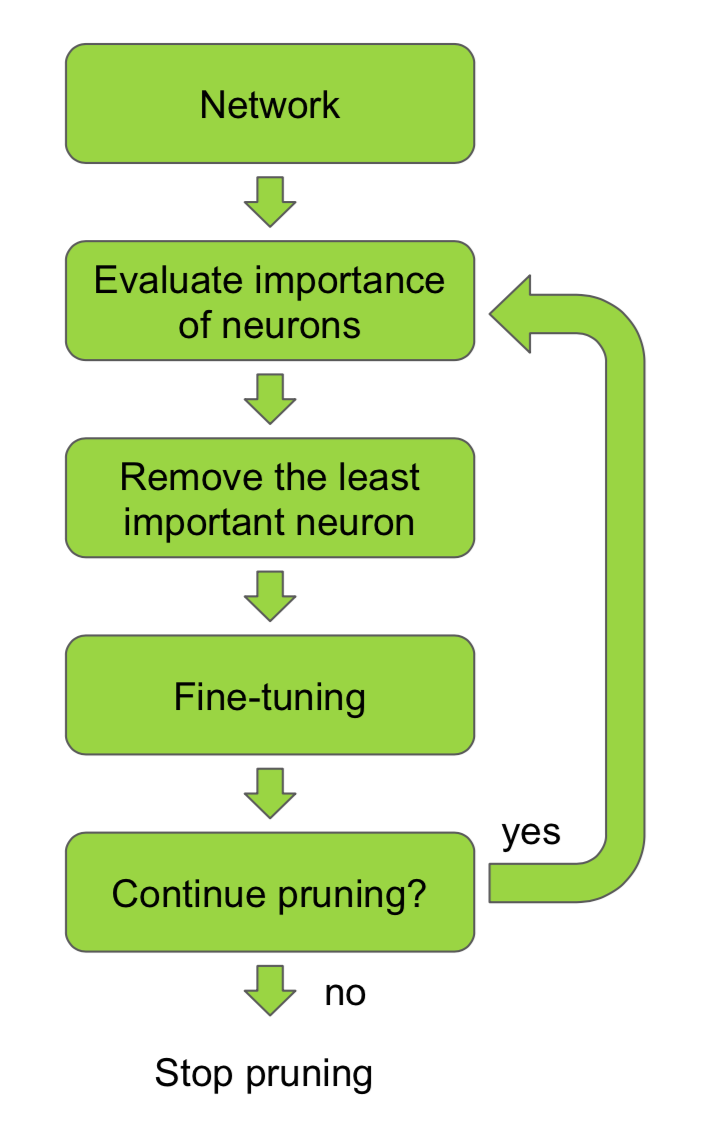
\includegraphics[width=4cm]{Figures/PruningMethod.png}
	\caption[Inference Optimisations]{Pruning method as a backward operator, presented in \cite{Molchanov2016}}
	\label{fig:PruningMethod}
\end{figure}

The last presented approach is \emph{quantisation} as it uses mixed-precision and uses it to optimise CNN models. This optimisation was closely studied since 2016 that was a year where many researchers studied the phenomenon. Starting in 2015 and 2016, Hubara, Courbariaux et al. \cite{Hubara2016, Courbariaux2015, Courbariaux2016} present the first works on \emph{QNNs}  and write the first training methodology for \emph{BNNs}.

Techniques have been presented the same year by Miyashita et al. \cite{Miyashita2016} to train \emph{QNNs}. In their work, they highlight a new logarithmic data representation to encode a neural network using 3-bits values. Their data representation consists of using \guille{non-uniform, base-2  logarithmic representation to encode weights, communicate activations and perform dot products}. They manage achieve higher classification accuracies than fixed-point at the same resolution and they propose a 5-bit representation that achieve higher test accuracy than 5-bit linear representation. Through their encoding, they manage to save space by encoding weights and activations in less space and save memory bandwidth by replacing the dot product (multiply accumulate) with a simpler operator for the logarithmic representation as shown on \emph{Figure} \ref{fig:DotProdLog}.

% LOG REPRESENTATION
\begin{figure}[htbp]
	\centering
		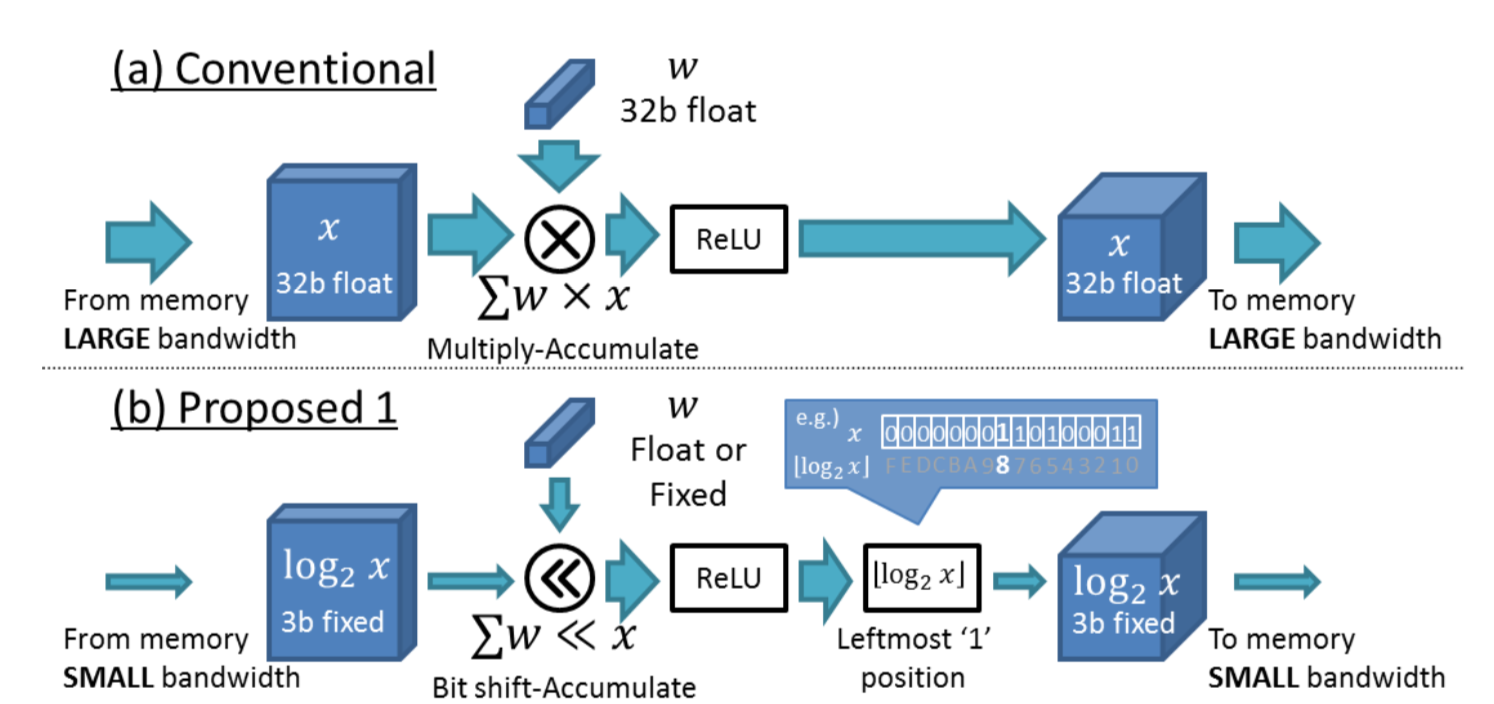
\includegraphics[width=12cm]{Figures/DotProdLog.png}
	\caption[Logarithmic Dot Product]{The Logarithmic way to perform Dot-Product \cite{Miyashita2016}}
	\label{fig:DotProdLog}
\end{figure}

Using yet another data representation, Micikevicius et al. \cite{Micikevicius2017} store weights, activations and gradients in IEEE half-precision nearly halving the memory requirements and speeding up the arithmetic. The authors propose three techniques to maintain the accuracy of the model. They maintain a single-precision copy of weights to accumulate the gradients, propose a loss-scaling to preserve low-magnitude gradients and use half-precision arithmetic that writes to single-precision arithmetic before writing the half-precision values to memory. A layer performs several operations in order to keep a high precision result, this behaviour is shown on \emph{Figure} \ref{fig:HPTraining}.

% LOG REPRESENTATION
\begin{figure}[htbp]
	\centering
		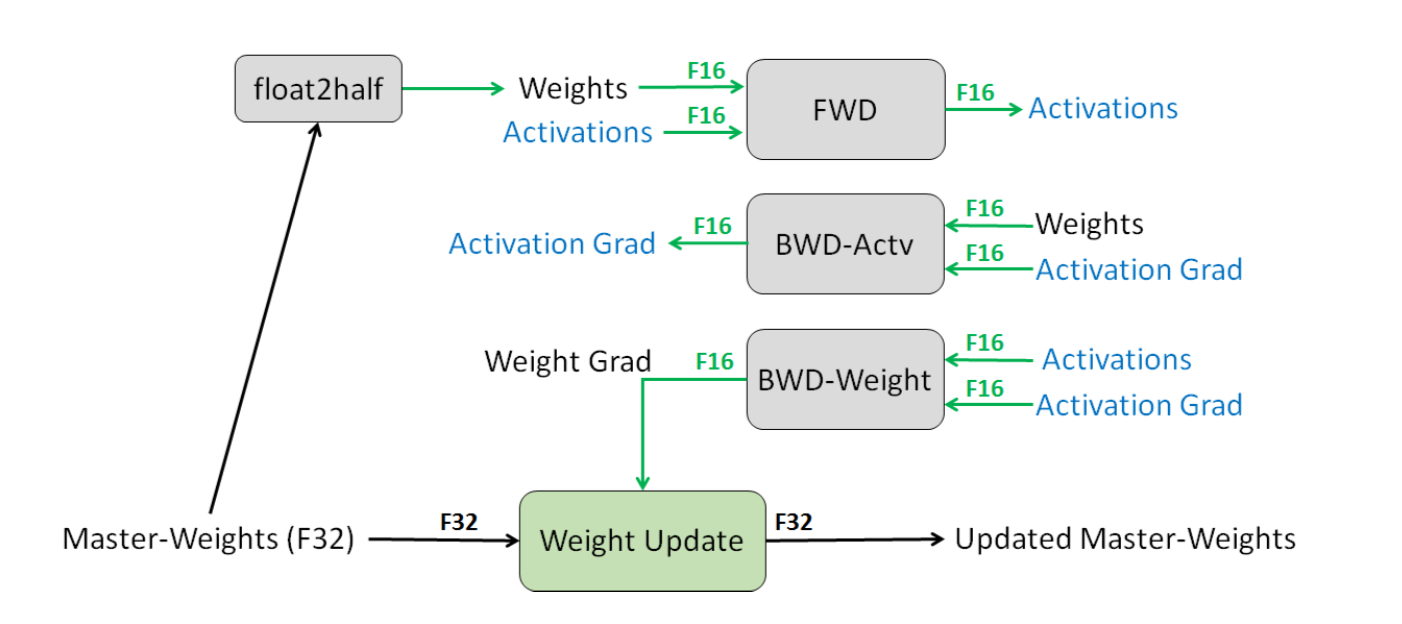
\includegraphics[width=10cm]{Figures/HPTraining.png}
	\caption[HPTraining]{Half-Precision Training  \cite{Micikevicius2017}}
	\label{fig:HPTraining}
\end{figure}

Rastegari et al. \cite{Rastegari2016} present \emph{Binary-Weights Networks}, on the same vein as Courabariaux et al. \cite{Courbariaux2016}. Their implementation however outperform the other of more than 16\% in top-1 accuracy. On the other hand, they present \emph{XNOR-Nets} that, for the first time, reduce dot-product operations to \emph{XNOR} operations followed by a \emph{Population Count (POPCount)} operator that counts the number of ones in the binarised vector. The \emph{XNOR-Nets} are using mostly bitwise operations to approximate convolutions and this enables a speed-up of approximately 58 times and enables \guille{the possibility of running state-of-the-art deep neural networks on CPU (rather than GPU) in real-time}.

Zhou et al. \cite{Zhou2016} present \emph{DoReFaNet}, a method to train neural network that have low bitwidth weights and low bitwidth activations. This is done by using low bitwidth gradients. During the backward pass, parameters gradients are quantised to low bitwidth numbers before being propagated to convolutional layers. They present a version of \emph{AlexNet} that has 1-bit weights, 2-bit activations that is trained from scratch using 6-bit gradients and manages to get 46.1\% top-1 accuracy on \emph{ImageNet}, a state-of-the-art performance.

Mixed-precision is extremely useful when dealing with \emph{inference} on low-space, low-energy hardware architectures. However, it can also be used to speed up the training times of deep neural networks on large datasets (such as \emph{ImageNet} for example). For now, training \emph{ResNet-50} on 8 Tesla P100 GPUs takes 29 hours \cite{He2016}. This time  impedes the research and development progress. Jia et al. \cite{Jia2018} present a novel mixed-precision training method along with an optimised all-reduce algorithm. Any neural network will have to use a version of an all-reduce algorithm, consisting of the sum of all the previous elements broadcasted to all the next elements. Using an optimised version of the algorithm will increase the performance of each layer separately and the whole system in the end. This method along with a \emph{Synchronised Stochastic Gradient Descent (SVG)} allows them to train the network extremely quickly on their setup (consisting of a cluster of 1024 Tesla P40 GPUs). Mixed-precision allowed them to speed-up the training to a point where they manage to train \emph{ResNet-50} in 15 minutes and \emph{AlexNet} in 4 minutes, both on the \emph{ImageNet} dataset.


%-----------------------------------
%	SECTION 3.3 - CNNs on FPGAs
%-----------------------------------

\section{CNNs on FPGAs}

Due to their heavy parallel affinity, CNNs can benefit from both GPUs \cite{Micikevicius2017, Jia2018, Kurth2018} and FPGAs \cite{Park2016, Liang2017, Colangelo2018, Jahanshahi2019, Bacchus2020} heavy parallelisation capabilities.
However, CNNs as stated in \cite{Jahanshahi2019}, \guille{CNN-based methods are computational-intensive and resource-consuming, and thus are hard to be integrated into embedded systems such as smartphones, smart glasses and robots}. FPGAs can counterbalance this issue by providing a tailored hardware representation of the CNN and making the most our of limited precision datatypes. They also appear as an in-between alternative over GPUs and under ASICs.

%--------------------------------------------
%	SUBSECTION 3.3.1 - Parallelisation Vectors
%--------------------------------------------

\subsection{Parallelisation Vectors}

Low-energy embedded systems can take advantage of the affinity of CNNs with parallelisation. This extensive concurrency can be used when parallelising from either \emph{Batch Parallelism} or \emph{Inter-Layer Parallelism}.

Batch size is an important parameter when looking at networks, it corresponds to \guille{a hyper-parameter that defines the number of samples to work through before updating the internal model parameters (weights)} \cite{MLMastery2019}. As stated in \cite{MLMastery2019}, the difference between a \emph{batch} and an \emph{epoch} is that an epoch consists of a full run through the training set while several batches can fit into an epoch. The batch size can divide the training in several types depending on the batch size:

\begin{itemize}
	\item \emph{Batch Gradient Descent}: Batch size = Size of the training set
	\item \emph{Stochastic Gradient Descent}: Batch size = 1
	\item \emph{Mini-batch Gradient Descent}: 1 $<$ Batch size $<$ Size of the training set
\end{itemize}

A CNN can simultaneously run the filters of the network on the instances of the same batch and obtain a significant acceleration when using batch processing. On the other hand, the structure of the network can be described as \guille{feed-forward}, meaning the output of layer $n$ is directly fed into layer $n+1$. A pipelined implementation can trigger the layer $n+1$ before the end of layer $n$ on selected instances.

The layers CONV are source of concurrency that can be exploited through the separation of the different planes the CONV layer uses (inter-FM), or the separation of the outputs of the layer (intra-FM). Moreover, the 3D-convolution can be expressed as a sum of 2D-convolutions that can be executed in parallel (inter-convolution) and the 2D-convolutions themselves can be pipelined concurrently (intra-convolution).

Many modern development frameworks implement a distributed version of optimisers and back-propagation to perform operations with \emph{MPI} or \emph{NCCL} for \emph{CUDA Tensors}. This allows both training and inference to be sped up by distributing their different heavy-load operations (multiply accumulate, dot-products, all-reduce, etc.). It also allows to separate the different instances from within the same batch to be run separately before gathering the resulting impact on the network parameters.

FPGAs run against several bottlenecks such as limited bandwidth and on-chip memory. However, due to their flexible nature, CNNs can be adapted to be run on them. Qiu et al. \cite{Qiu2016} show in their state-of-the-art study that the Convolutional layers are computationally-centric and Fully-Connected layers are memory-centric. This means that using any of the two layers will have to bring a concern on the associated bottleneck it holds as well.

%---------------------------------------------------------
%	SUBSECTION 3.3.2 - Training and Inference Optimisations
%---------------------------------------------------------

\subsection{Training and Inference Optimisations}

FPGAs provide an in-between solution between GPUs and ASICs. They can be used in both \emph{Training} and \emph{Inference} in order to process the different instances of the dataset they are being fed. This subsection will present the different training and inference optimisations that can be brought on FPGAs. As said earlier, the \emph{Inference} step is a critical spot of CNN implementations as it is required each time a new instance is presented to the system whereas the \emph{Training} step can be done once and for all. Increasing the performance of this step is crucial and can be done in several ways. First, the memory bandwidth is the bottleneck of several FPGA implementations. High number of memory reads or high number of weights stored result in a loss of performance. A caching strategy is often a nice answer to this kind of issues.

Next, the literature presents several optimisations strategies that will help the CNN perform best on an FPGA. Exporting a CNN to an FPGA consists in finding the most efficient way to map the CNN on the hardware architecture of the FPGA. The main strategies are listed beneath and presented in \emph{Figure} \ref{fig:InferenceOpt}. Several solutions found in the literature present combination of different strategies to perform best on a given architecture. Several methods have already been presented in the \emph{Optimisation Methods} subsection such as \emph{Pruning}, \emph{Compression} or \emph{Quantisation} with an FPGA note. \emph{Pruning} still has an FPGA implementation as presented by Fujii et al. \cite{Fujii2017} as well as an accelerator model proposed by Kang et al. \cite{Kang2019}. However, more FPGA-specific methods exist.

\begin{figure}[htbp]
	\centering
		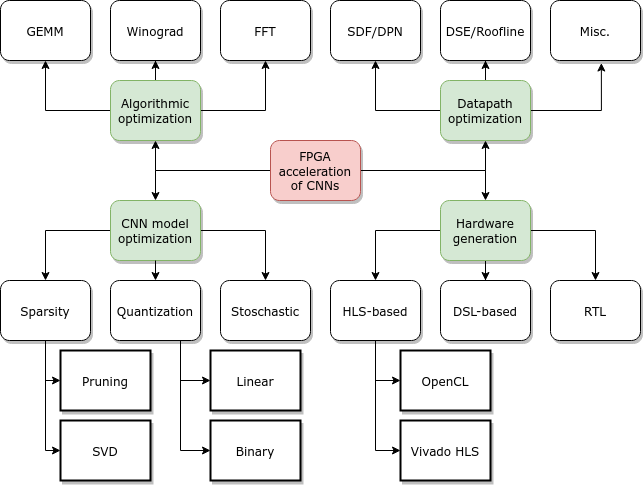
\includegraphics[width=.75\textwidth]{Figures/InferenceOpt1.png}
	\caption[Inference Optimisations]{Methods to accelerate an FPGA implementation \cite{Abdelouahab2018}}
	\label{fig:InferenceOpt}
\end{figure}

The main strategies specific to FPGAs are linked to \emph{Hardware Generation} and \emph{Data-path optimisations}. The first one, \emph{Hardware Generation}, depends on the way the configurable hardware will be used and tuned. As shown in \emph{Figure} \ref{fig:InferenceOpt}, several methods exist to reconfigure an FPGA. Some use \emph{High Level Synthesis} through either OpenCL or Vivado. These different frameworks and accelerators will be the focus of subsection \ref{fpga_framework}. On the other side, the \emph{Data-path optimisations} mainly revolve around the idea of loop optimisation. Several methods can be applied to the execution of nested loops to perform better on an FPGA. Loop optimisation comes in two different shapes: \emph{loop unrolling} and \emph{loop tiling}.

Unrolling a loop accelerates its execution at the cost of resource utilisation. Loop tiling consists of modifying the order of the different embedded loops in order to have the most expensive operations come all-together. These operations are \emph{DRAM (external memory)} accesses where the weights are stored since the FPGA cannot store them all with on-chip memory. An example of loop tiling can be seen on \emph{Figure} \ref{fig:LoopTiling}.

The settings of unroll and tiling factors will directly determine the number of \emph{Processing Elements (PE)} and their associated computing resources as well as the amount of DRAM accesses.

% Loop Tiling
\begin{figure}[htbp]
\centering
\begin{minipage}{.48\textwidth}
\begin{lstlisting}[style=CInputStyle]
// Ll: Layer
for (int l=0;l<L,l++){
// Lb : Batch
for (int b=0;b<B,l++){
// Ln: Y Depth
for (int n=0;n<N;n++){
// Lv: Y Columns
for (int v=0;v<V,v++){
// Lu: Y Raws
for (int u=0;u<U,u++){
// Lc: X Depth
for (int c=0;n<C;c++){
// Lj: Theta Columns
for (int j=0;j<J,j++){
// Lk: Theta Raws
for (int k=0;k<K,k++){
  Y[b,l,n,v,u] += X[b,l,c,v+j,u+k] *
        Theta[l,n,c,j,k]
}}}}}}}
\end{lstlisting}
\end{minipage}
\hfill
\begin{minipage}{.48\textwidth}
\begin{lstlisting}[style=CInputStyle]
for (int n=0;n<N;n+=Tn){
for (int v=0;v<V,v+=Tv){
for (int u=0;u<U,u+=Tu){
for (int c=0;n<C;c+=Tc){
  // DRAM: Load in on-chip buffer the tiles
  // X[l,c:c+Tc,v:v+Tv,u:u+Tu]
  // Theta [l,n:n+Tn,c:c+Tc,j,k]
  // Process on-chip tiles
  for (int tn=0;tn<Tn;tn++){
  for (int tv=0;tv<Tv,tv++){
  for (int tu=0;tu<Tu,tu++){
  for (int tc=0;tn<Tc;tc++){
  for (int j=0;j<J,j++){
  for (int k=0;k<K,k++){
    Y[l,tn,tv,tu] += X[l,tc,tv+j,tu+k] *
            Theta[l,tn,tc,j,k];
  }}}}}}
  // DRAM: Store output tile
}}}}
\end{lstlisting}
\end{minipage}
\caption[LoopTiling]{Loop Tiling Example \cite{Abdelouahab2018}}
	\label{fig:LoopTiling}
\end{figure}

Now if we look more closely on \emph{Quantisation} methods applied to FPGAs, the literature present several works:

Colangelo et al. \cite{Colangelo2018} present a CNN mapping to a reconfigurable architecture in order to use sub 8-bit activation and weights. In order to use binary- or ternary-weighted neural networks, they cap their sizes to respectively 1 and 2-bits. Using this type of limited numeric precision can only be fully optimised with FPGAs and the authors show that they manage to get an optimisation of \guille{the bandwidth, memory, power and computation savings}.
uning
Zhao et al. \cite{Zhao2016} propose \emph{F-CNN}, a framework to train CNNs on FPGAs. Their design makes available highly customisable modules that will be optimised to maximise performance under the constraints of bandwidth and hardware resources. The authors state that the introduction of mixed-precision will be the next step of optimisation of their design. Moreover, the use of they prove their design is more performant than CPUs and less expensive in terms of energy than GPUs. \emph{F-CNN} reconfigures a streaming datapath at runtime to cover the training tasks for the various layers in a CNN.

Jahanshahi et al. \cite{Jahanshahi2019} propose a CNN accelerator tool. It generates the hardware description for a CNN to be programmed on a target FPGA. The software uses an API the developer can use to enter the available resources. The software will then generate the hardware description and run a simulation to adjust the precision and minimise the classification error. The whole system is shown to be more performant on a half-precision fixed-point representation rather than using single-precision floating-point data: 3\% accuracy loss in exchange for 15.75x speedup.

The even more agressive vision of quantisation with binary parameters as set by Courbariaux et al. \cite{Courbariaux2016} was conducted on GPUs but their FPGA counterpart have been developed later on. Liang et al. \cite{Liang2017} present a BNN implemented on an FPGA and the benchmarked results show an improvement in speed and energy efficiency over other computing platforms.


%--------------------------------------------------------
%	SUBSECTION 3.3.3 - FPGA Frameworks
%--------------------------------------------------------

\subsection{FPGA Frameworks}\label{fpga_framework}

In 2016, the same year \emph{QNNs} began to gain attraction and credibility, FPGA frameworks emerged to take advantage of FPGA capabilities along with mixed-precision. The first works in the fields are \emph{YodaNN} \cite{Andri2016} and \emph{F-CNN} \cite{Zhao2016}. Andri et al. set up \emph{YodaNN}, an accelerator optimised for \emph{BNNs} and one of the first implementations. Zhao et al. \cite{Zhao2016} designed F-CNN, the first FPGA framework to train CNNS. Later on, Wang et al. \cite{Wang2018} developed a design flow for extremely low-bit neural networks that focuses on quantisation in both training and FPGA deployment. They aimed at strict resources and power constraints in order to provide a design to the developer.

The next year, two initiatives are launched in order to perform an automatic mapping of a CNN down to its hardware counterpart on an actual hardware architecture. \emph{fpgaConvNet} is created by Venieris et al. \cite{Venieris2017}. It automates the mapping of CNNs on FPGAs using application-level needs (throughput, latency or multiobjective criteria). It uses a paradigm called \emph{Synchronous Dataflow (SDF)} and defines a set of \emph{SDF} transformations in order to efficiently explore the design space. \emph{fpgaConvNet} implements four different transformations the network will be run through: \guille{\emph{graph partitioning}with reconfiguration, coarse-grain \emph{folding}, fine-grained \emph{folding} and weights \emph{reloading}}. Those four different transformations can be seen on \emph{Figure} \ref{fig:fpgaConvNetTransformations} respectively (a), (b), (b) and (c).

\begin{figure}[htbp]
	\centering
		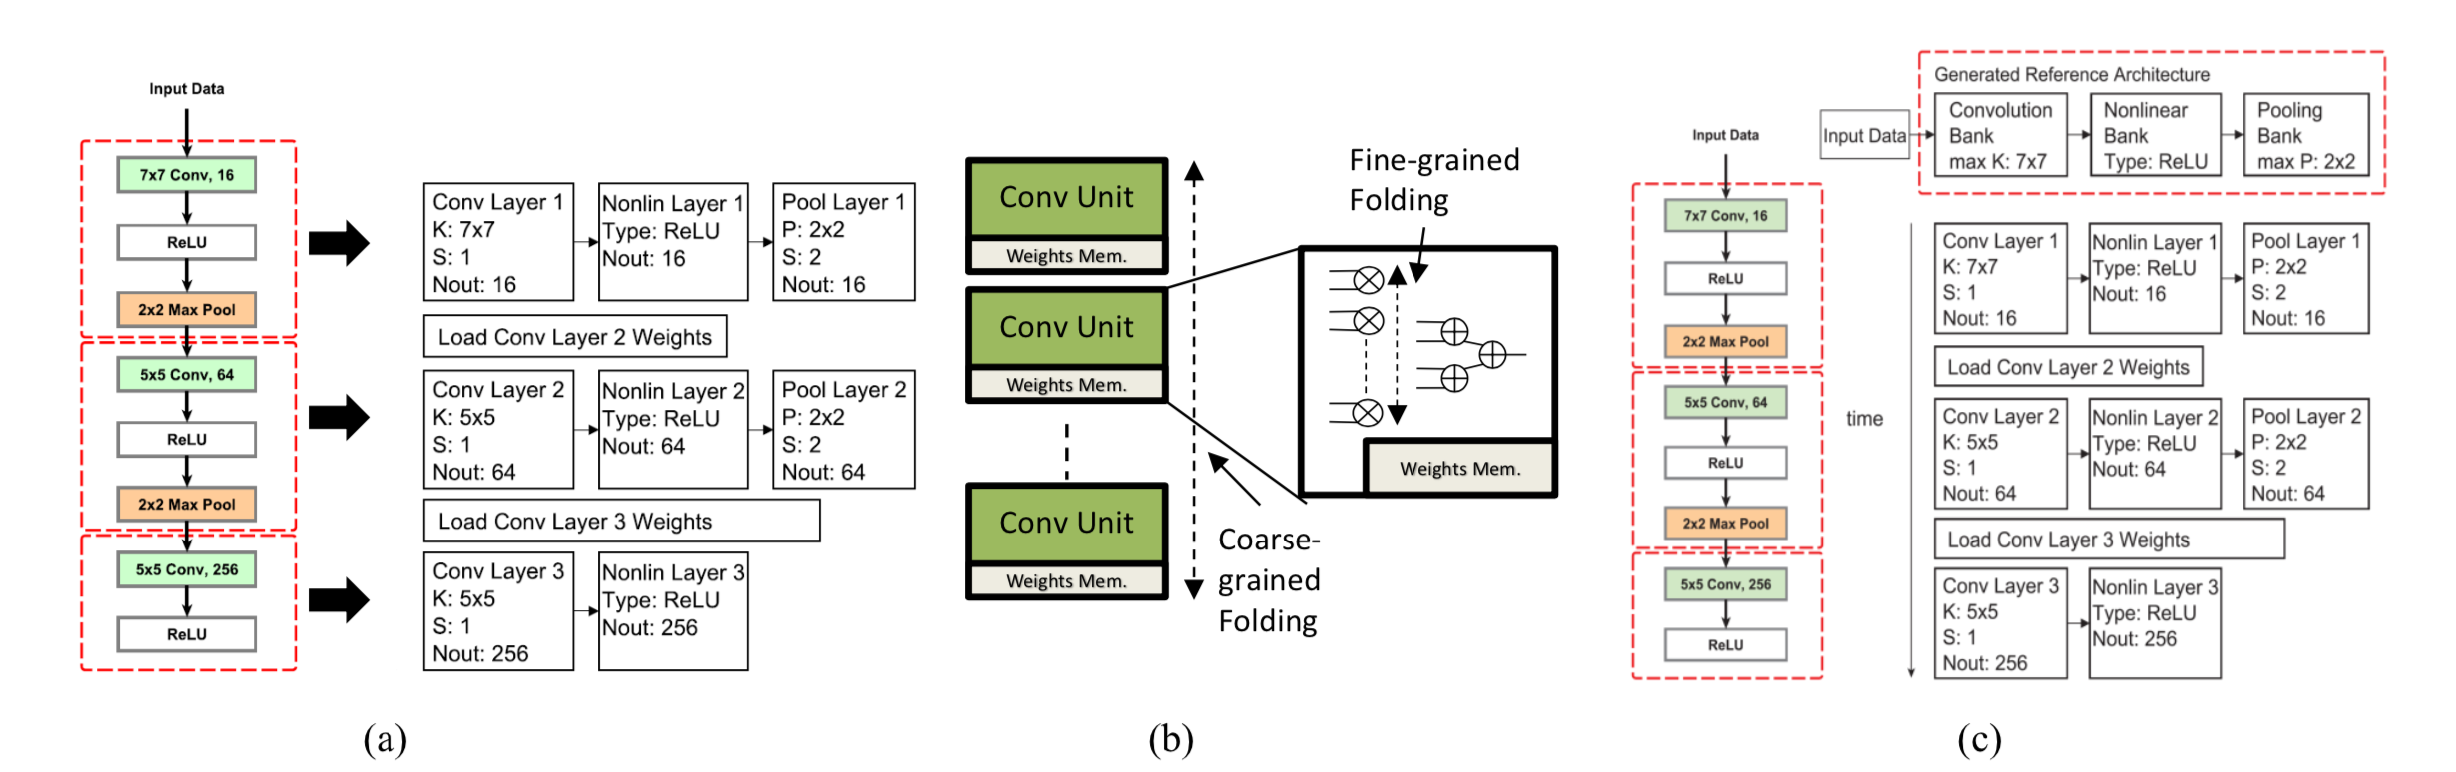
\includegraphics[width=\textwidth]{Figures/fpgaConvNetTransformations.png}
	\caption[Inference Optimisations]{Different transformations used by \emph{fpgaConvNet} \cite{Venieris2017}}
	\label{fig:fpgaConvNetTransformations}
\end{figure}


The tool will separate the CNN into different subgraphs that will be tailored specifically to the target architecture. The execution of each subgraph requires a reconfiguration of the FPGA and \emph{fpgaConvNet} performs a batch-processing of the subgraph in order to amortise reconfiguration times. This transformation is called \emph{graph partitioning}. Next, \emph{coarse-grain folding} enables the tuning of the number of coarse units for each layer. It spans a fully parallel implementation down to a single, time-shared unit. Then, \emph{fine-grained folding} allows the configuration of the dot-product implementation in the convolutional units of a layer. It spans a fully parallel implementation down to a single , time-shared multiply-accumulate unit. Finally, the \emph{weights reloading} is similar to the first transformation in the sense that it will separate the network in several parts but will this time single flexible reference to all the weights of the network. This allows a layer to use the weights of the last layer without reloading them in memory.

In the other hand, \emph{FINN} \cite{Umuroglu2017a} has been developed as an open-source framework by the FPGA manufacturer Xilinx. It works as a network compression tool especially tailored for FPGAs and have been actively under development with extensions to quantised networks \cite{Blott2018} or Long Short-Term Memory (LSTM) networks \cite{Rybalkin2018}. It has been developed in order to propose a complete workflow to its users. First, another tool developed by Xilinx can be used in order to train quantised networks, \emph{Brevitas}. This tool produces a network in an intermediate representation with annotation for the FPGA framework. \emph{FINN} loads this intermediate representation and, in the same way \emph{fpgaConvNet} would do, runs the network through a series of different transformations. \emph{Figure} \ref{fig:FinnWorkflow} presents the whole workflow.

\begin{figure}[htbp]
	\centering
		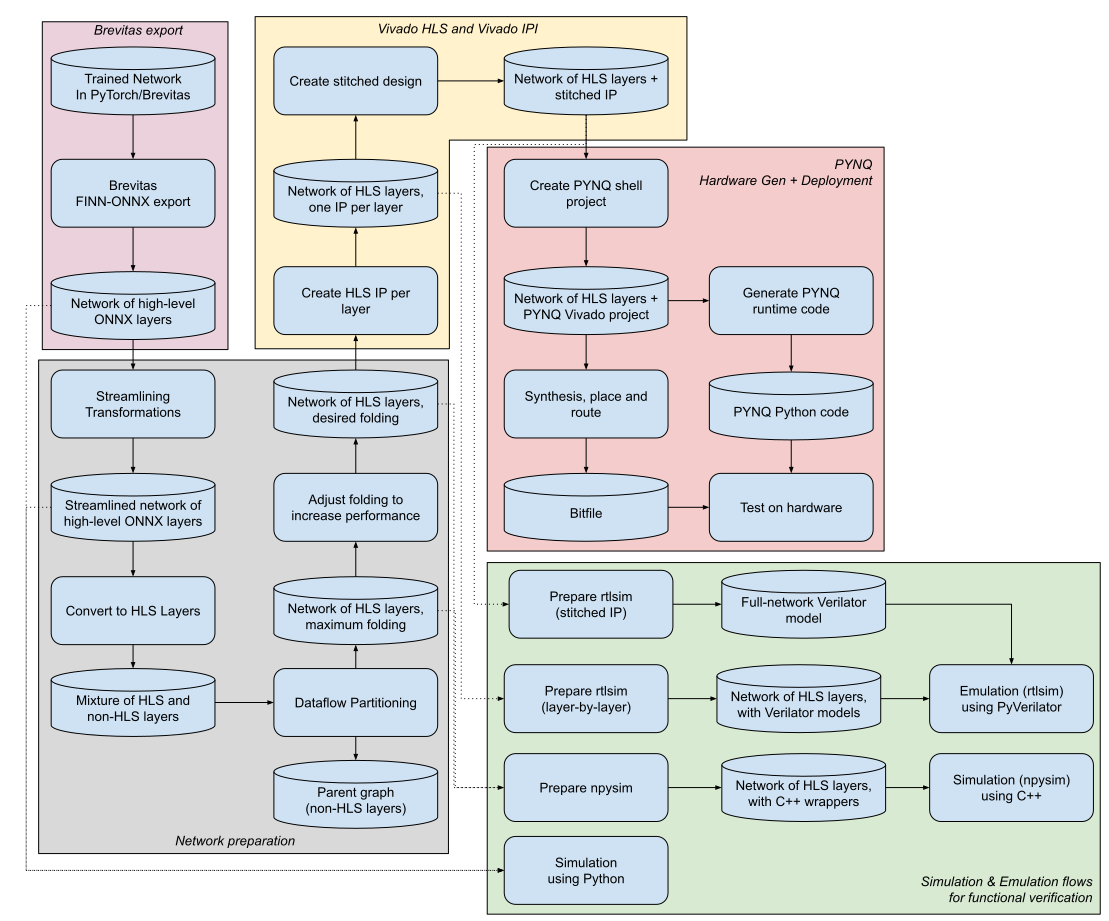
\includegraphics[width=\textwidth]{Figures/FinnWorkflow.png}
	\caption[Inference Optimisations]{FINN workflow as presented in \cite{Umuroglu2017a, Blott2018}}
	\label{fig:FinnWorkflow}
\end{figure}

The first transformations are called \emph{tidy-up} and consists of renaming the different nodes in the intermediate representation, renaming the tensors and infering shapes and data types. Next, another series of transformations arrives under the name of \emph{streamlining}, or a way to eliminate floating-point operations. It moves the operations around and collapses them into \emph{multithresholding} nodes. Next, the layers are converted into \emph{High-Level Synthesis (HLS)} layers, seprating the overall graph into a mixture of \emph{HLS} nodes and \emph{non-HLS} nodes. Then, the graph is split in two parts, one containing \emph{HLS} nodes that will be executed on the board while others are kept as they are. This step is called \emph{dataflow partitioning}. Finally, a \emph{folding} step is provided, where parameters such as the number of \emph{PEs (Processing Elements)} or \emph{SIMDs (Single Instruction Multiple Data)} can be tuned. The network will then be processed layer by layer and converted to a hardware counterpart. This counterpart consists of a stitched \emph{IP (Intellectual Property)} composed by other \emph{IPs}, one per layer. \emph{IPs} are custom blocks that can be processed by an FPGA.

An interesting difference between the two frameworks is the \emph{FINN} ability to simulate the steps during the workflow. This verification (as shown in the green bottom-left part of \emph{Figure} \ref{fig:FinnWorkflow}) can be performed in three different ways: a simulation using Python after the network is exported in intermediate representation, a simulation in C++ when the network contains the \emph{HLS} nodes and an emulation using \emph{PyVerilator} when the different IP blocks (one per layer) are generated. \emph{FINN} also comes with a dedicated trainer for networks. This trainer provides \guille{drop-in} replacements for PyTorch layers.

In 2019, Ding et al. \cite{Ding2019} propose a \guille{Resource-aware, efficient quantisation framework} for object detection on FPGAs. They present an extension and automation of the YOLO model used in the object detection field. Jahanshahi et al. \cite{Jahanshahi2019} present TinyCNN, a modular CNN framework using 16-bit fixed-point data. Zhao et al. \cite{Zhao2019} present Tomato, \guille{a framework designed to automate the process of generating efficient CNN accelerators}. Tomato uses different arithmetics and precisions within each Convolutional layer. This is the first multi-precision multi-arithmetic auto-generation framework for CNNs.

Between all these different frameworks, \emph{FINN} seems to be the one that encounter a growing community. This may be due to the fact that the initiative is pushed by Xilinx, a well-known FPGA manufacturer. Their tools provide interconnection, whether it is between their boards and FINN or the integration with their GUI \emph{Vivado} and \emph{Vitis}.

%------------------------------------------------------
%	SUBSECTION 3.4 - Takeaway from the Literature Review
%------------------------------------------------------

\section{Takeaway from the Literature Review}
In this \emph{Background} and \emph{Literature Review}, the focus went from the background of number representation, machine learning and hardware architectures to the underlying link between them, mixed-precision. The next part showed the different ways to both use mixed-precision in serious scientific computations and apply it to practical machine learning. The final parts present the works made to optimise both training and inference for neural network on different architectures. The final point was to present the existing tools to port a mixed-precision network to a \guille{by-default} mixed-precision architecture, FPGAs.

Benchmarking and optimisation are extremely important topics in the field of machine learning when it comes to evaluation of a new set up, architecture or optimisation methods. Extensive benchmarking has been done on well-known network architectures or datasets and this provides an easy insight on what went better and what went worse. However, very few effort has been put together to compare development frameworks implementation between them. This translates in a lack of answers from industrials or companies to choose concretely for a solution before running into an artificial intelligence or machine learning project. For now, the question is \guille{Which company from the GAFA would you like to support by using their framework?} rather than actual performance. The difference also comes from the tools developed on top of these frameworks.

When looking at optimisation methods, parameters are empirically chosen and few benchmarks exist to test them and their reliability. Several articles from the literature often propose an empirical choice in parameters size along with the architecture and performance they got out of the experiment. Bacchus et al. \cite{Bacchus2020} benchmark the trade-offs between training-time, hardware efficiency and accuracy in QNNs while varying the size of the parameters. The work proposed could be extended with new frameworks, architectures and  datasets. The experiment could be reconducted on different architectures and datasets in order to confirm or invalidate the sweet spots found. An extension to \emph{fpgaConvNet} or \emph{Brevitas} (with PyTorch) could widen the benchmark. In fact, if binarisation is known to be effective when coming from a 32-bit floating point representation. However, little data covers the impact of the quantisation of weights, as opposed to the impact of the quantisation of activations and what would a sweet spot be. Many factors come into play: network architecture, dataset, optimiser, loss function, quantisation, transformations pre- and post-training as well as hardware deployment methods.

There is room for benchmarking state-of-the-art implementations of \emph{QNNs} on FPGAs and their associated frameworks. FINN seems to be the one that chose to be developed in an open-source way, with an extension to a well-known framework (PyTorch) and the use of a common intermediate representation. Creating a scalable benchmark that could be given a network architecture, dataset, quantisations of weights and activations as well as training time would allow proper testing of a framework and show the flexibility of such a framework.
